\chapter{Background and Literature Review}
\label{ch:background}
%A literature and technology review, leading up to the problem that is tackled—you should show a knowledge and awareness of the relevant literature and/or technologies. You shouldn't just give a descriptive list of other work: you should organise the work that you review in an appropriate scheme, show connections and contrasts between the work, point out the strengths and weaknesses of existing work, and where appropriate clearly identify what the current state-of-the-art approaches are to the problem.
% The dissertation needs to have a background chapter/literature review explaining the context of the project. For example, if the project is using machine learning, there has to be an explanation of how the machine learning approach used in the project works. If the project is on an e-voting system, there has to be an overview of existing e-voting systems, how they work, and the dissertation should show understanding of the main challenges in implementing a safe and secure e-voting system. 
% Explaining what your project does that is new or is better than existing work in the same field.

\section{Embeddings}\label{sec:embeddings}
For \acrshort{ai} models to be able to process text, a numerical representation is required. Improvements in these numeric representations have significantly contributed to the field of \acrfull{nlp}, particularly in recent years. Initial models used integer IDs to represent words by deriving an integer value from the frequency of a word occurring. This is known as a bag-of-words approach and is based on the work of \citet{Zellig}. Although variations of this have been employed, such as 'n-grams' (collections of n successive words), this approach is limited in its ability to capture the semantic information within a language \citep{Monisha}. In addition, these methods face challenges when dealing with large corpora as the model dimensionality is dependent on the number of unique words. 

\subsection{Word2vec}\label{sec:embeddings_word2vec}
An alternative approach known as word2vec was developed by \citet{mikolov2013efficient} and aimed to overcome both of these limitations by building on the work of \citet{bengio2000neural}. It is a technique which uses two-layer neural networks (see Section \ref{sec:background_anns}) to produce learned word embeddings so that words that have similar usage in the training corpus are close (have a similar cosine similarity/small cosine distance) in the embedding vector space. Therefore, these vectors are superior to integer IDs in containing semantic detail. We can observe this by considering a common example using the vector representations of the words king, man, and woman ($w_K$, $w_M$, and $w_W$ respectively), it can be shown that:
\begin{equation*}
    \begin{aligned}
        w_K - w_M + w_W &\approx w_Q \\
        King - Man + Woman &\approx Queen
    \end{aligned}
\end{equation*}
Where $w_Q$ denotes the vector representation for `Queen', which is the word with the smallest cosine distance to the above calculation \citep{allen2019analogies}.

\cite{mikolov2013efficient} proposed two possible approaches: one is to use the surrounding words to predict the `current' one (\acrfull{cbow}) and the other is where the `current' word is used to predict the surrounding ones (Skip Gram). A key feature of this approach is that each vector characterises the context of the word by considering neighbouring tokens, as opposed to just the word itself \citep{li2018introduction}. However, this approach cannot handle words that are not in the training corpus. Additionally,  words with contrasting sentiments, such as ``good” and ``bad”, are closely located in the vector space \citep{sivakumar2020review} as they are often used in similar contexts, highlighting a key limitation of the \acrshort{cbow} or Skip Gram approach.

% NOT FOR WORD2VEC: A key benefit of this approach is that vectorised word embeddings have the potential to detect and classify words that are previously unseen to the model \citep{Rudkowsky}.

\subsection{Context}\label{sec:embeddings_context}
Word2Vec and other similar embeddings such as \acrshort{glove} \citep{Pennington} have long been the industry standard. However, these embeddings fail to take context into account. For instance, such models provide one vector per word and, consequently, cannot differentiate between a `fun fair' and a `process being fair', for example. This stems from disregarding word order and, importantly, generating a sole vector representation per word. Therefore, it is essential to generate contextualised embeddings to represent words. Transformer models such as \acrfull{bert} were developed by \citet{devlin2019bert} in response to the original `Attention is All You Need' paper \citep{vaswani2017attention} to overcome this limitation, taking into account both left- and right- context (i.e. words before and after the current word).

Entire sentence and paragraph embeddings can also be generated, which can be used for sentiment analysis. Averaging non-contextual word embeddings is a crude way to achieve this, but Transformer models typically used attention mechanisms to extract the semantic meaning of a sentence or paragraph and generate a high-dimension embedding vector \citep{langchain}.

%(this uses its placement within a sentence using the sin/cos functions? What about the sentence placement - which sentence it is?) Therefore we can have similar representations of fair/unbiased and fair/carnival.

%\acrfull{bert} was developed in order by \citet{devlin2019bert} to overcome this limitation, taking into account both left and right context (i.e. words before and after the current word). Previous models such as \acrshort{elmo} used \acrshort{cnn} and \acrshort{lstm} architecture \citep{peters2018deep}, but \acrshort{bert} dispensed with this technology, using a series of stacked encoders and is trained using masked-language modeling and next sentence prediction. By using Transformers instead of  

%Use BERT's pre-training (Self-supervison) to generate contextual encodings for words? And then use fine-tuning/feature-based approach for use with another model.

%BERT can understand previously unseen/rare words by breaking them into sub-words (`wordpieces') \citep{wu2016googles}.

\section{Early Chatbots}\label{sec:background_early_chatbots}
The earliest chatbots used rule-based logic to respond to textual inputs. One of the earliest chatbots was Eliza, created in 1966 by researchers at \acrshort{mit} to pass the Turing Test \citep{zemvcik2019}. It used pattern matching to be able to construct human-like replies \citep{Luka}. However, the responses were often formulaic and predictable. These systems faced limitations due to the intricate nature of language, as it is highly difficult and inefficient to generate rules to handle every possible query. Many developments have been made since these early frameworks, with the adaptations outlined below.

%The development of \acrfull{ai} and \acrfull{nlp} meant that chatbots began to learn from data and

\section{\acrlong{ann}s}\label{sec:background_anns}
\acrlong{ann}s (\acrshort{ann}s) are part of a branch of machine learning called deep learning, with machine learning itself being a branch of \acrlong{ai}. \acrshort{ann}s seek to provide solutions to a wide range of classification, pattern recognition and prediction problems and are used extensively in image recognition and \acrfull{nlp} tasks \citep{Abiodun}. Inspired by the human brain, they are analogous to the nervous system; they take an input and, using a complex set of neurons, seek to identify an output response \citep{Bishop}. They do this by learning from examples, in a similar way to humans. For example, \acrshort{ann}s can be used to predict whether an image contains a pizza or a football.

\subsection{Structure}\label{sec:background_anns_structure}
Neural networks take a series of inputs (via the input layer) and seek to predict the output (via the output layer). To achieve this, they often contain several `fully connected' hidden layers of a pre-determined size consisting of neurons and nodes that hold weights and biases. The size of the input layer is determined by the number of attributes that the model has available to it, and the size of the output layer is determined by the classification/prediction problem. 

\begin{figure}[h]
    \centering
    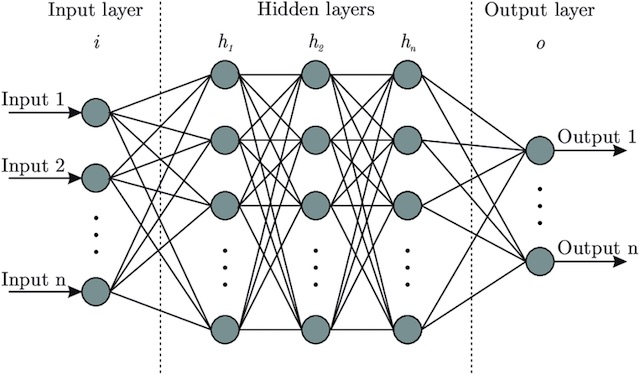
\includegraphics[height=5.5cm] {paper/images/neural_network_structure.jpeg} % ,trim={0 0 0 0cm},clip
    \caption{Typical Neural Network Structure \citep{Shukla}}
    \label{fig:neural_network_structure}
\end{figure}

This structure is shown in Figure \ref{fig:neural_network_structure}, where each grey circle denotes a node, and each interconnecting line denotes a weight between two nodes. As can be seen, each node is connected to every node in the next layer (in a fully connected layer), and the value of each node in the next layer is a weighted sum of the values of the nodes in the previous layer and their corresponding weights (and sometimes a bias term) \citep{Bishop}. The weights, therefore, determine how much information is passed on to each node in the next layer. The weights are analogous to the strength of the connection of biological neurons, and the bias is analogous to the firing threshold in the human brain \citep{rathi2020dietsnn}.

\subsection{Activation Functions}\label{sec:background_anns_activation_functions}
The value in each node of a neural network is typically transformed by an activation function, often Sigmoid or \acrfull{relu}. The former ensures that the values are non-linearly scaled to be between 0 and 1 using $f(x) = \frac{1}{1+e^{-x}}$, whereas the latter truncates values that were below 0 to be 0 using $f(x) = max(0, x)$. Consequently, the range of a sigmoid activation function is $(0, 1)$ and the range of a \acrshort{relu} activation function is $[0, \infty]$. These activation functions, along with some other common ones, are shown in Figure \ref{fig:activation_functions}.

\begin{figure}[h]
    \centering
    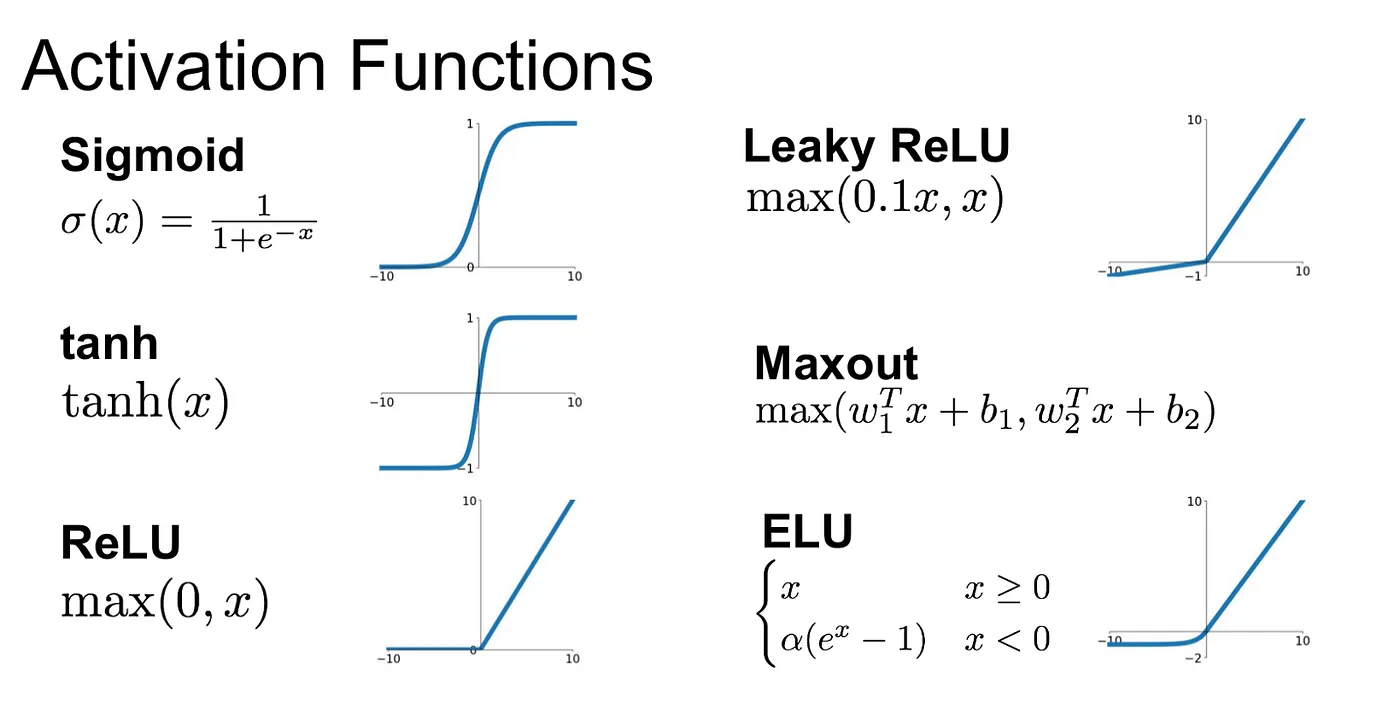
\includegraphics[height=5.5cm,trim={0 0 0 3.5cm},clip]{paper/images/activation_functions.png}
    \caption{Activation Functions Used in Neural Networks \citep{Udofia}}
    \label{fig:activation_functions}
\end{figure}

This process is continued for each of the (fully connected) hidden layers until the network has calculated the values for each of the nodes in the output layer. This will typically be a proportion which, in the case of next sentence prediction, denotes the likelihood of that specific word being the next word in the sentence.

\subsection{Learning}\label{sec:background_anns_learning}
The learning in neural networks occurs in training the weights that connect each of the nodes. \acrlong{ann}s use a technique known as Forward Propagation to calculate the predicted output from a given input. Initially, the weights in the network are randomly assigned \citep{Bishop}, meaning that the model has essentially no prior predictive power. For each example data point the network calculates the values for each of the nodes in the output layer; these denote ``the probability that the given input fits into each of the pre-set categories" \citep{Yathish}. This process is repeated for each of the training examples and is known as Forward Propagation. 

The predicted values are subsequently compared against the expected (true) value, and the model computes the error (the difference between the predicted and true values). This error is fed into a loss function (E), which is a measure of the inaccuracy of the model; the aim is to minimise the loss function. For most classification problems, a cross-entropy (log loss) function is used to compare the difference between the actual value ($y_i$) and the predicted value ($\hat{y_i}$) for each of the prediction classes (of size $N=n^L$, where L is subscript and not an exponent):

$$E = -\sum_{i=0}^{n^L-1} y_i*log(\hat{y_i})$$

Once the value for the loss function has been calculated, the model seeks to update weights and biases in each layer, using a process called backpropagation \citep{Rumelhart, maths2015Nielsen}. We can define the following notation:

$a_j^L$: \textit{The output value of the jth node in the Lth layer (once the activation function has been applied)}

$w_{jk}^L$: \textit{The weight connecting the jth node in the Lth layer and the kth node in the (L-1)th layer}

$b_j^L$: \textit{The bias applied to the jth node in the Lth layer}

$z_j^L = w_j^L a_j^{L-1} + b_j^L$: \textit{The value of the jth node in the Lth layer}

We can therefore say that $a_j^L = \sigma(z_j^L)$, where $\sigma$ denotes the activation function.

The backpropagation process begins by computing the rate of change of the cost function with respect to each of the weights (holding other weights constant) because we are seeking to minimise the cost function. This is given by $\partial E/ \partial w_{jk}^L$.
% ,\quad \forall  i \in [1,n^L]$$ where $n^L$ denotes the size of the current layer (L is subscript and not an exponent).
By using the chain rule, we can expand this expression:
$$\frac{\partial E}{\partial w_{jk}^L} = \frac{\partial z_j^L}{\partial w_{jk}^L} \frac{\partial a_j^L}{\partial z_j^L} \frac{\partial E}{\partial a_j^L}$$ % \; can work for spacing
Similarly, we can calculate $\partial E/ \partial b_j^L$ and $\partial E/ \partial a_j^{L-1}$. Using these, the gradient of the cost function can be computed and used to update the parameters above so that the cost function is reduced. Gradient Descent is the process of adjusting the parameters in the `direction' indicated by the gradient of the cost function, such that the loss function is reduced. The size of the adjustment is called the `learning rate', and this affects how quickly the model adjusts its parameters.

This adjustment is applied to all of the network's layers as part of the backpropagation process and for each of the training examples. One iteration of the combined training process is known as an Epoch (Forward Propagation, Cost Calculation, and Backpropagation using Gradient Descent) \citep{Sharma}, and this is applied recursively until the loss function is sufficiently small. The smaller the learning rate, the more epochs are typically required to reach the minimum loss required. Once all of the epochs are completed, and the training process has reached a local minimum, the model is ready to produce predictions. However, it may not necessarily have reached a global minimum, meaning that predictions may not be completely optimal.

\section{\acrlong{rnn}s}\label{sec:background_rnns}
\acrlong{rnn}s (\acrshort{rnn}s) are a form of neural network used for sequential data. They take each element of the sequence one at a time and use the current and previous values to predict future ones. They can crudely be thought of as ``very deep feedforward networks in which all the layers share the same weights'' \citep{Yann}. This is depicted in Figure \ref{fig:rnn_architecture}, where the input is processed sequentially ($x_{t-1}, x_{t}, x_{t+1},\ldots$), and information from the previous state is used to make the prediction in the current state ($h_{t}$). However, when backpropagation is used to train the network, problems are often encountered.

\begin{figure}[h]
    \centering
    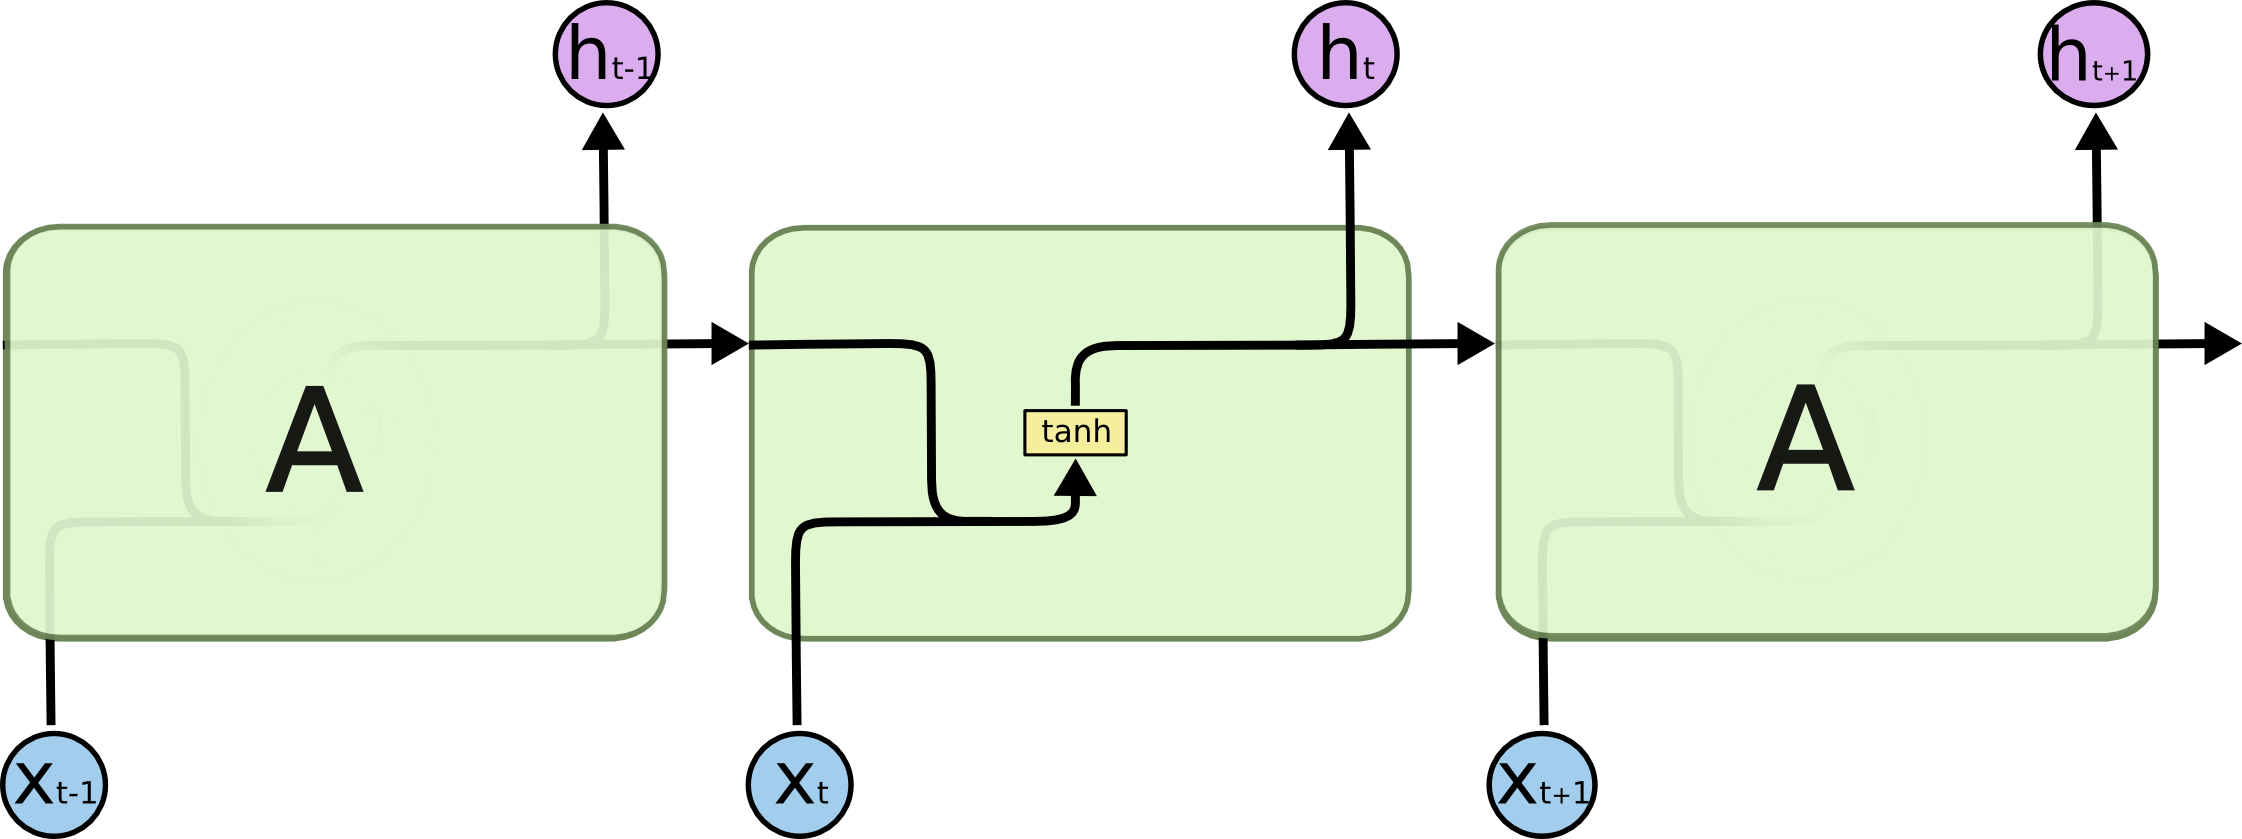
\includegraphics[height=4.5cm,trim={0 0 0cm 0cm},clip]{paper/images/rnn.png}
    \caption{Architecture of a \acrlong{rnn} \citep{olah2015understanding}}
    \label{fig:rnn_architecture}
\end{figure}

A common problem with training neural networks is the vanishing/exploding gradient problem \citep{hochreiter1997long}. This can occur in deep neural networks but is particularly common in \acrshort{rnn}s, as the same weights are used in each iteration. The exploding gradient problem is where the model weights become exponentially large, which causes the model weights to become \acrshort{nan}. Alternatively, because of the recurrent structure of the model, there can be a tendency for model weights to `vanish' and tend to 0. This causes the model to have short-term memory because it fails to capture long-term dependencies \citep{chung2014empirical}. In addition to this, in both cases, the loss function is not minimised because the weights cause the loss function to either overshoot or never reach the global/local minimum.

\subsection{\acrlong{lstm} Cells}\label{sec:background_lstms}
\acrfull{lstm} networks are a type of \acrlong{rnn} which were developed by \citet{hochreiter1997long} to overcome the vanishing/exploding gradient problem. They are depicted in Figure \ref{fig:lstm_architecture} where, instead of one simple layer (as in Figure \ref{fig:rnn_architecture}), there are three layers with different activation functions. \acrshort{lstm} networks use a sigmoid ($\sigma$) activation function for each of their three `gates' (forget gate, input gate, and output gate) to determine how much of the long-term memory is maintained and to update both the long-term and short-term memory in each cell. The first (most left-wise neural network layer in Figure \ref{fig:lstm_architecture} is the `forget gate'. The `input gate' refers to the second layer, which is subsequently combined with a layer with a tanh activation function to update the long-term memory. The final layer is the `output gate', which also uses a sigmoid activation function. By using this structure, \acrshort{lstm} networks overcome the vanishing and exploding gradient problem because they control how much the gradient vanishes using the `forget gate' \citep{Gers}.

\begin{figure}[h]
    \centering
    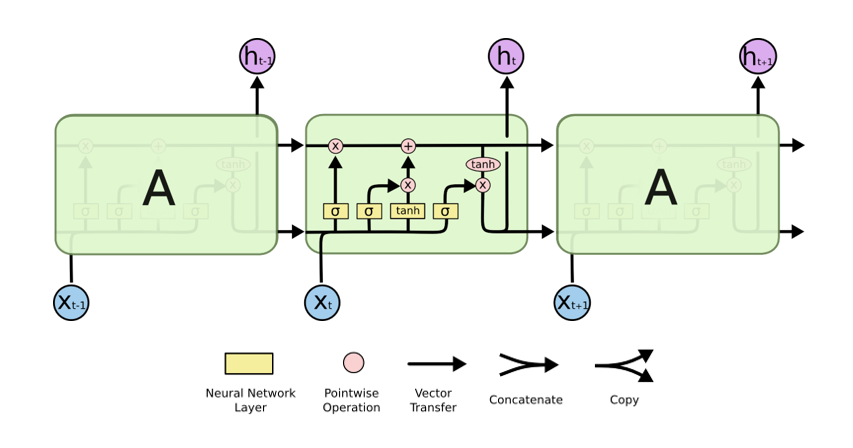
\includegraphics[height=7.5cm,trim={0 0 0 0cm},clip]{paper/images/lstm.png}
    \caption{Architecture of a \acrlong{lstm} Cell \citep{olah2015understanding}}
    \label{fig:lstm_architecture}
\end{figure}

\subsection{\acrlong{gru}s}\label{sec:background_grus}
Another similar model to \acrshort{lstm}s is the \acrfull {gru}, with an architecture based on just two gates (reset gate and update gate). It was developed in 2014 by \citet{cho2014learning} and provides a simpler architecture than the \acrshort{lstm} model. This model is shown in Figure \ref{fig:gru_architecture}, which shows how the flow of information is held using a `hidden state' and the two gates (the neural network layers with sigmoid activation functions) determine how much information it remembers or forgets. The update gate determines how much of the memory it retains, and the reset gate determines how much of the memory it forgets.

\begin{figure}[h]
    \centering
    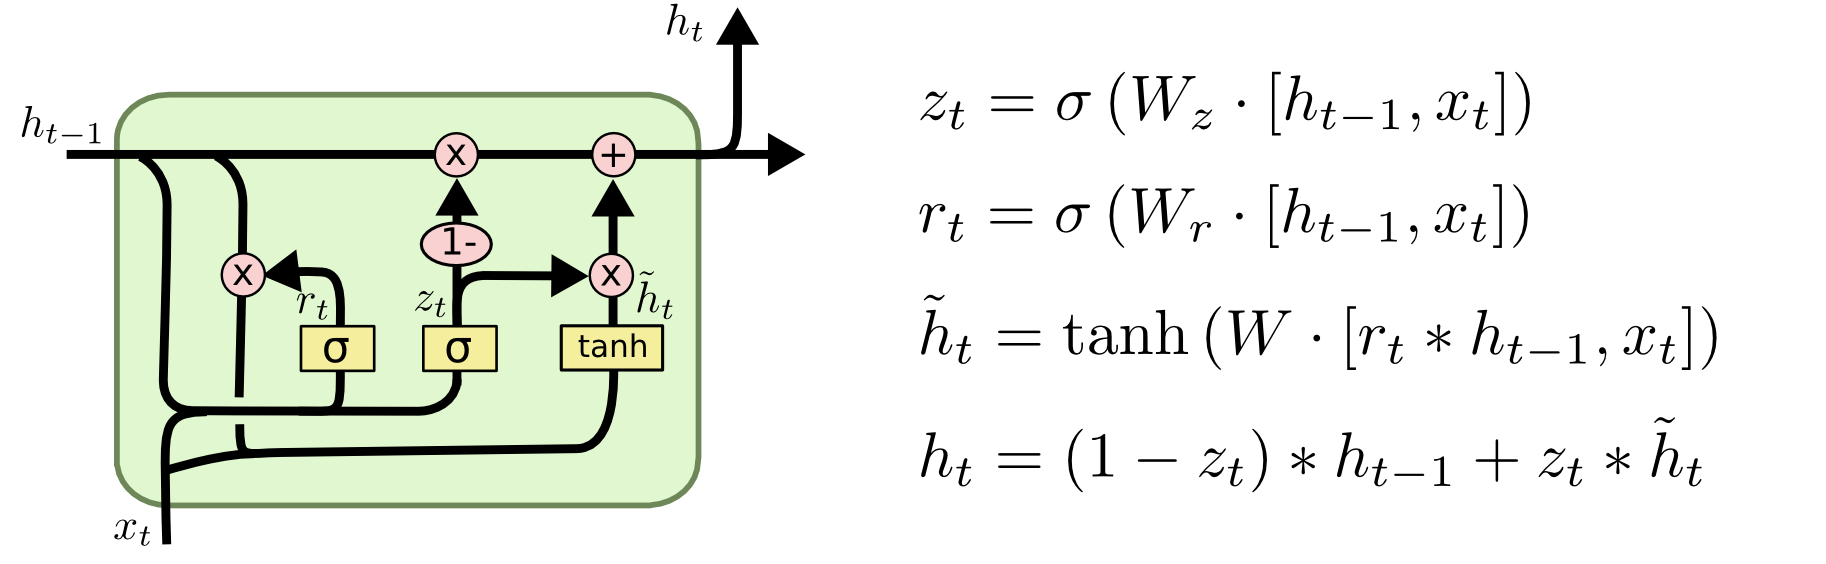
\includegraphics[height=4.5cm,trim={0 0 12cm 0cm},clip]{paper/images/gru.png}
    \caption{Architecture of a \acrlong{gru} \citep{olah2015understanding}}
    \label{fig:gru_architecture}
\end{figure}

The \acrlong{gru} has become popular due to its simplicity relative to the \acrshort{lstm} architecture, but \acrshort{lstm} cells and \acrshort{gru}s often perform similarly effectively. However, it has been noted in the literature that \acrshort{gru}s generally outperform LSTM networks on sequences that are short and less complex, whereas \acrshort{lstm} models are typically preferred for longer and more complex sequences \citep{cahuantzi2023comparison}. This is often attributed to the \acrshort{lstm} model's ability to better capture long-term dependencies in sequences, which often means it is preferred for language modelling \citep{Irie2016}. However, both models (and vanilla \acrshort{rnn}s generally) can only capture forward dependencies, due to their sequential nature. For example, with the sentence `Joel read a book about a bass that was owned by a fisherman', using only the first seven words, you would not know whether the word `bass' refers to the fish or the instrument. It is only with the latter parts of the sequence that you can determine the context and therefore the bass was owned by the fisherman and not the musician. Therefore, models which only capture forward dependencies will miss any potential inference based on future words. 

\subsection{Bidirectional \acrlong{rnn}s}\label{sec:background_bidirectional_rnns}
To overcome this limitation, Bidirectional \acrshort{rnn}s were developed by \citet{Schuster} and are a combination of two \acrshort{rnn}s (see Section \ref{sec:background_rnns}). One \acrshort{rnn} processes information in the usual chronological manner, while the other processes it in reverse time order. The model is trained simultaneously on both of these and seeks to minimise the loss function for both time directions concurrently. This allows the model to capture the future context in sequences, which is particularly important in \acrshort{nlp} implementations because the context of words is typically derived from future words.

All of the above models (\acrshort{rnn}s, \acrshort{lstm}s, and \acrshort{gru}s) require sentences to be processed sequentially, so can take a long time to train especially when there are long strings to process, and can have convergence issues due to vanishing/exploding gradients \citep{vaswani2017attention, Lipton}. We will now explore an alternative model which seeks to solve this.

% \section{\acrlong{cnn}s}
% \label{sec:background_cnns}

% A popular varation of the vanilla neural network is the \acrfull{cnn}. It uses convolutions for feature extraction which is then fed into a fully connected neural network for the classification \citep{Budiharto}, and is efficient as convolutions perform well on \acrshort{gpu}s. They have been used to produce \acrfull{sota} results in image classification \citep{krizhevsky2017imagenet}, but can also be successfully applied to \acrshort{nlp} tasks \citep{kim2014convolutional}.

% The architecture is outlined in Figure \ref{fig:cnn_architecture}. The model begins by convolving multiple matrix filters over the concatenated vector representation of the input sequence (often word2vec; see Section \ref{sec:embeddings_word2vec}) in order to extract
% patterns in the input. Each convolutional layer typically contains a non-linear activation function (Section \ref{sec:background_anns_activation_functions}), after which pooling is used to reduce dimensionality without losing the most important information \citep{Severyn2015UNITNTD}. Typically, max pooling is used. The final layer is a fully connected softmax layer which outputs the probability distribution of the various output classes (e.g. sentence sentiment).

% \begin{figure}[h]
%     \centering
%     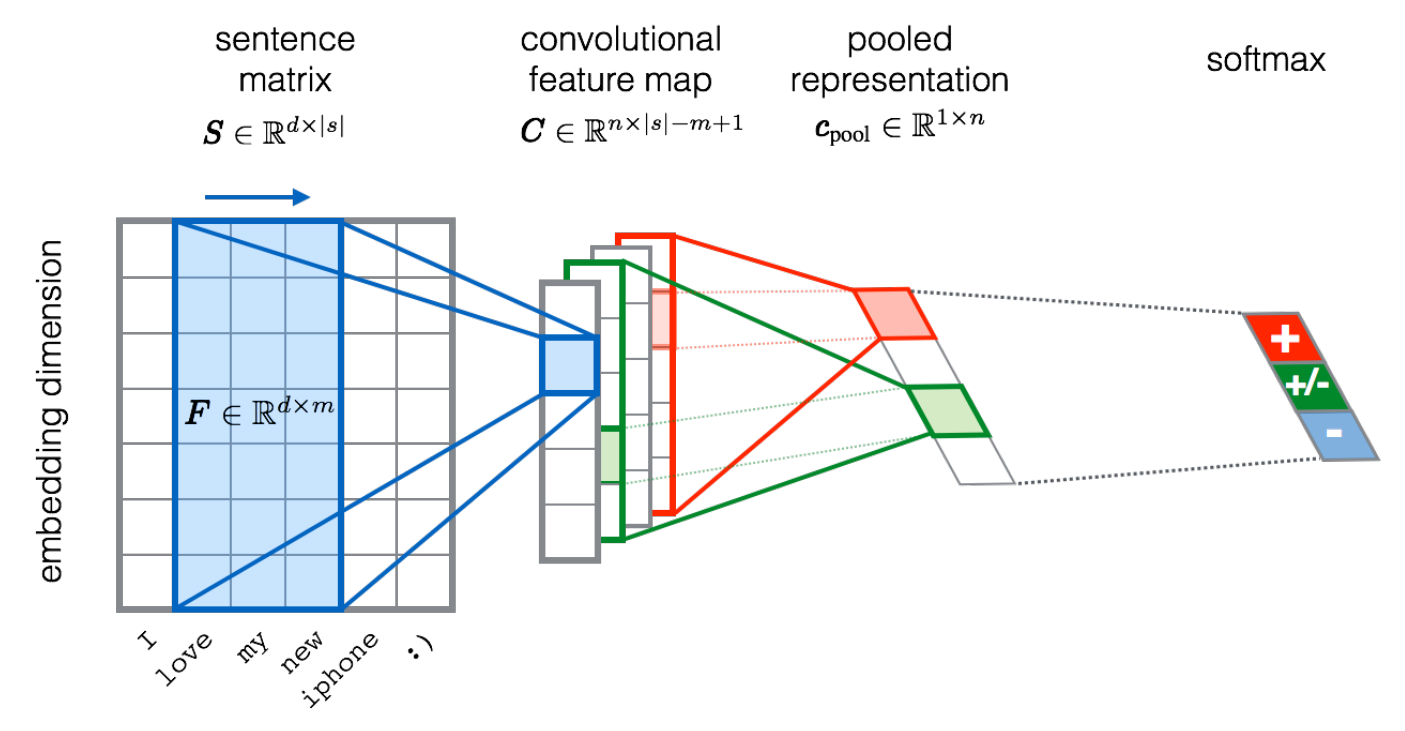
\includegraphics[height=6cm,trim={0 0 0cm 0cm},clip]{paper/images/cnn.png}
%     \caption{Architecture of a \acrlong{cnn} \citep{Severyn2015UNITNTD}}
%     \label{fig:cnn_architecture}
% \end{figure}

% Need to critically analyse CNNs and other architectures rather than simply write about them

\section{Transformers}\label{sec:background_transformers}
Transformers were introduced in \citeauthor{vaswani2017attention}'s `Attention Is All You Need' paper (\citeyear{vaswani2017attention}). The authors proposed a sequence-to-sequence model which uses six stacked encoders and decoders, though subsequent models often use varying numbers of encoders and/or decoders. The strength of Transformers lies in their ability to process all words in a sentence simultaneously (the sequential nature of \acrshort{lstm} networks made them slow to train), and their ability to retain context from much further back in the sequence \citep{vaswani2017attention}.

While there are many variations, the initial model architecture is shown in Figure \ref{fig:transformer_architecture}. It begins by taking initial embeddings such as word2vec (Google's \acrshort{bert} uses wordpiece tokenisation to easily handle out-of-vocabulary words \citep{wu2016googles}), and applies a vector containing positional encodings for each word (using $sine$ and $cosine$ functions). These positional encodings are then passed into the encoder block.

\begin{figure}[h]
    \centering
    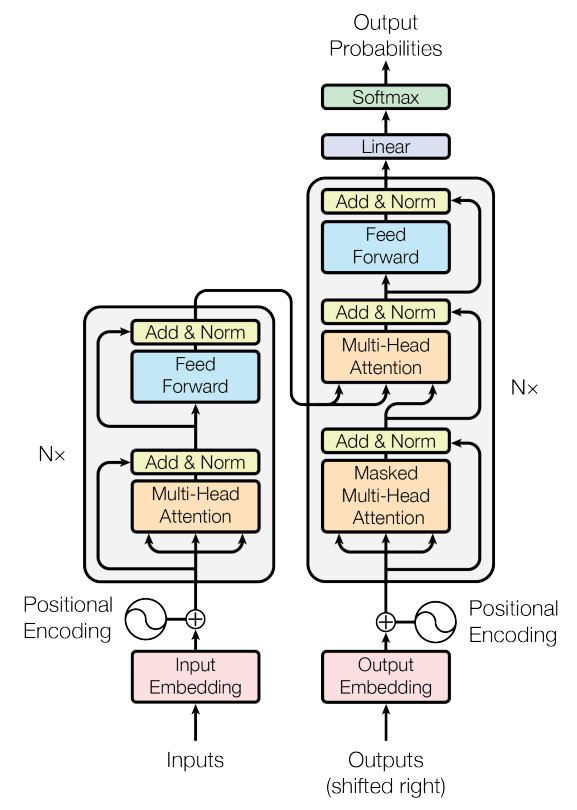
\includegraphics[height=10cm,trim={0 0 0cm 0cm},clip]{paper/images/transformer.png}
    \caption{Architecture of a Transformer model \citep{vaswani2017attention}}
    \label{fig:transformer_architecture}
\end{figure}

\subsection{Encoder}\label{sec:transformers_encoder}
An encoder consists of a multi-headed attention block combined with a feed-forward neural network, both of which are followed by layer normalisation. Firstly, the positional encoding vectors are used to calculate self-attention vectors, which specify how each word relates to every other word in the sequence. Each self-attention vector can be independently passed into the neural network, enabling the model to leverage \acrshort{gpu} parallelisation and significantly reduce training time. Finally, the encoder outputs a contextualised vector, which can be intuitively conceptualised as containing the `meaning' of the word within its context.

\subsection{Decoder}
The decoder uses a similar architecture to the encoder but uses masking to prevent the model from `seeing ahead' in the sentence. For example, to translate the phrase ``Esta es una tesis fantástica'' from Spanish to English, the model should not see any word ``tesis fantástica'' when calculating the self-attention for the phrase ``Esta es una''. This means that the model has unidirectional-context (typically only left-context). Once the masked multi-headed attention vectors have been calculated, the decoder combines this with the output from the encoder using another multi-headed attention block. Finally, this information is passed into a feed-forward neural network to produce the prediction for the next word in the sequence until an end-of-sentence token (\texttt{<EOS>}) is produced.

\subsection{Variations}
There are multiple variations of the Transformer architecture.
They broadly fit into three categories. The first is autoencoding (bidirectional) models which use stacked encoders (e.g. \acrshort{bert}: \citet{devlin2019bert}); the second is autoregressive (left-context) models which use stacked decoders (e.g. \acrshort{gpt}: \citet{radford2018improving}); the third is a combination of both, using both stacked encoders and decoders (e.g. \acrshort{bart}: \citet{lewis2019bart}), and these are known as sequence-to-sequence models. 

\acrshort{bert} excels at text classification and question answering. The model was released by Google in October 2018, and its success comes from utilising between 12 and 24 stacked encoders ($\sim$110 and $\sim$340 million parameters, respectively). These enable the model to extract high-dimensional semantic information about the text, and therefore either classify the sentiment or extract words which answer a question.

\acrshort{gpt} was released after \acrshort{bert}, with the first version of \acrshort{gpt} (\acrshort{gpt}-1) released by OpenAI in June 2018. The model excels at being able to generate contextually-aware text in natural, human-sounding form, due to its use of many stacked decoders. Subsequent versions, such as \acrshort{gpt}-2 and \acrshort{gpt}-3, were improvements on the original model and used to develop ChatGPT, which was released in November 2022 \citep{ChatGPTrelease}. However, the strength of \acrshort{gpt} is also one of its main criticisms; it is trained to generate text using statistical patterns and distributions in its training data, but this can result in the generation of plausible but false content. This method of training also results in the perpetuation of bias. For example, OpenAI ran the \acrshort{seat} \citep{may2019measuring} and Winogender \citep{rudinger2018gender} benchmarks to identify any potential bias in their model and found that \acrshort{gpt} tends to associate positive sentiment with European American names when compared to African American names, and can be prone to generating content associated with negative stereotypes of black women \citep{openAIembeddings}. This is caused by the model learning patterns from its training data which itself contains harmful content.

\acrshort{bart} was released after these models by Facebook AI Research in October 2019. \acrshort{bart} incorporates both bidirectional encoders and auto-regressive decoders, making it one of the best models for extractive question answering \citep{pearce2021comparative}. However, \acrshort{bart} also suffers from the same criticisms as \acrshort{gpt}, resulting in potentially false yet plausible content. \acrshort{bart}, along with the above variations of the Transformer architecture, is typically pre-trained using a very large corpus of information, and can subsequently be fine-tuned for downstream tasks, such as question answering, translation, or text generation. This is known as transfer learning, where fine-tuning pre-trained models can be completed using much smaller custom datasets, as the model utilises existing knowledge gained during the pre-training phase.


Transformer models are highly effective in being able to generate natural-sounding content and can be fine-tuned to complete a variety of tasks. They are more effective at retaining context than previous models and can process entire sentences simultaneously as opposed to sequentially (see Sections \ref{sec:background_bidirectional_rnns} and \ref{sec:transformers_encoder}). However, they still require many improvements to ensure that they generate factually accurate and safe content.

\section{Implementations}\label{sec:background_implementations}
There have been several recent attempts to produce reliable chatbots using \acrfull{sota} Transformer technology. The literature identifies two angles of approach. The first is to use fine-tuning, typically \acrfull{mlm}, to embed the knowledge into the model weights. The second is to find relevant paragraphs of information and subsequently provide this to the model by using the input message. It is important to note that, at the time of writing, \acrshort{gpt}-3.5 Turbo and \acrshort{gpt}-4, which power ChatGPT \citep{ChatGPTrelease} are not available for open-source fine-tuning. Only \acrshort{gpt}-2 its predecessors are available on open-source platforms. Therefore, while Khan Academy and a limited number of other companies are in the process of creating and trialling a knowledgeable chatbot \citep{khanAcademy}, this will not discussed in detail as it will not be accessible for most applications. 

The first of the above two approaches is \acrfull{mlm}. \acrshort{mlm} is used to extract the semantic information contained within the training text by updating model parameters to accurately predict masked words given the context in surrounding non-masked words. The partially masked sentence is taken as an input (e.g. ``I love natural [MASK] processing") and the model seeks to accurately predict the masked token (which in the above example is ``language"). However, this is not designed to be efficient for factual recall. OpenAI in their documentation note that ``fine-tuning is better suited to teaching specialized tasks or styles, and is less reliable for factual recall'' \citep{openai_cookbook_qa_embeddings}. Furthermore, models that rely only on model weights to provide factual, accurate answers often suffer from ``hallucination", which is a term the literature uses to refer to model responses which are confident and realistic-sounding but inaccurate \citep{manakul2023selfcheckgpt}. As a result, this approach is not recommended for `teaching' the model specific information.

The second approach involves using a document store, which can be implemented as part of either the pre-training or fine-tuning process. \citet{documentStoreGuu} proposed a retrieval-augmented pre-training model which uses relevant texts (from Wikipedia) to assist with the prediction of masked tokens, and penalised any poor document retrieval by the model. This is outlined in Figure \ref{fig:document_store}, where the retrieved document is used to pre-train the model to predict the masked token. However, this approach is not possible for most applications, because it requires huge amounts of data and processing power. Instead, most applications will require the use of models that have already been pre-trained. 

\begin{figure}[h!]
    \centering
    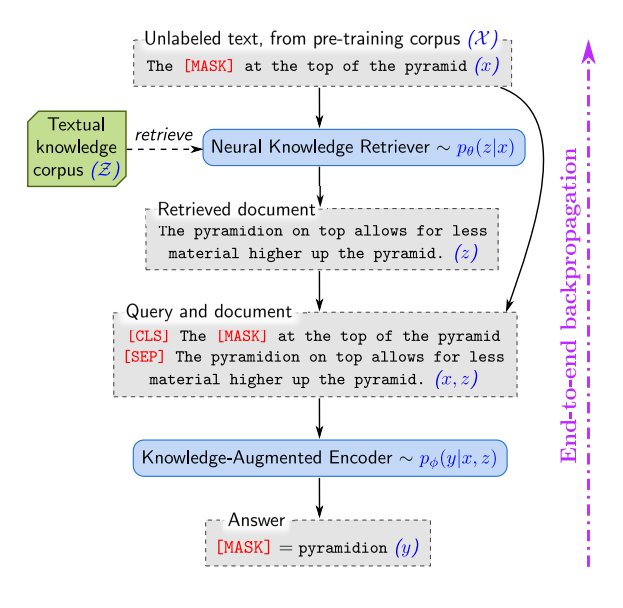
\includegraphics[height=8cm,trim={0 0 0cm 0cm},clip]{paper/images/document_store.png}
    \caption{Pre-training of a Retrieval-Augmented Language Model \citep{documentStoreGuu}}
    \label{fig:document_store}
\end{figure}

It is therefore more efficient for most applications to instead have a separate retriever which uses a semantic search (e.g. using the cosine similarity of sentence/paragraph embeddings). This approach is recommended by OpenAI for use with their \acrshort{gpt}-3.5 Turbo model \citep{openai_cookbook_qa_embeddings}. They describe the general knowledge embedded in the model as ``long-term memory'' and outline how providing relevant passages within an input message is akin to providing the model with ``short-term memory'' that yields more accurate and reliable answers. As a result of this, the development of relevant packages is underway, with early versions of an open-source Python package \texttt{LangChain} already available \citep{langchain}. By comparing the semantic similarity (e.g. cosine similarity) of a query and potentially thousands of relevant passages, the most relevant ones can be into a pre-trained model with a query, and the model can be fine-tuned to provide an answer. 

There are limitations to this approach, however. Firstly, the accuracy of any model is limited to its ability to extract (natural-sounding) answers from a piece of text. Such a model can either be achieved by fine-tuning an open-source pre-trained model, or by using an already fine-tuned model that is adept at question-answering. Secondly, any model will be constrained by a maximum amount of text it can read at once, placing an upper bound on the amount of information it can use to produce an answer. However, this approach is still preferred in the literature, due to the frequency of ``hallucination'' as a result of relying solely on model weights.


% Prior to the use of Transformer models, an alternative approach was used by \citet{Chen22} to create an extractive, domain-specific chatbot using a Deep \acrlong{cnn} (an \acrshort{lstm}-\acrshort{cnn} model), but this architecture cannot generate answers in natural language anywhere near as effectively. Therefore, this project seeks to provide a framework for a chatbot which can generate answers in natural language with a high degree of accuracy and reliability.

% Why search is better than fine-tuning: GPT can learn knowledge in two ways: Via model weights (i.e., fine-tune the model on a training set) and Via model inputs (i.e., insert the knowledge into an input message). Although fine-tuning can feel like the more natural option—training on data is how GPT learned all of its other knowledge, after all—we generally do not recommend it as a way to teach the model knowledge. Fine-tuning is better suited to teaching specialized tasks or styles, and is less reliable for factual recall. As an analogy, model weights are like long-term memory. When you fine-tune a model, it's like studying for an exam a week away. When the exam arrives, the model may forget details, or misremember facts it never read. In contrast, message inputs are like short-term memory. When you insert knowledge into a message, it's like taking an exam with open notes. With notes in hand, the model is more likely to arrive at correct answers. 

% Also:  In general, search-based systems do best on questions that have a simple lookup, and worst on questions that require multiple partial sources to be combined and reasoned about. https://github.com/openai/openai-cookbook/blob/main/examples/Question_answering_using_embeddings.ipynb


% IBM Watson was famously developed to compete on the quiz show Jeproady! and beat the then-champions to win 1st prize https://web.archive.org/web/20130616092431/http://www.jeopardy.com/news/watson1x7ap4.php

% question answering chatbots have gone from extractive question answering to generative question answering, where they use probabilities to generate text. By learning the patterns and semantics of language, it can generate human-like responses. Initially, Markov Chains were used to generate the most probable characters or words in the output (e.g. HeX) \citep{Luka, Ahmad}.

%"A comparative study of CNN and RNN for NLP explored by Yin et  al. [http://arxiv.org/abs/1702.01923] shows that RNN performs better than CNN in most of the NLP tasks" https://journalofbigdata.springeropen.com/articles/10.1186/s40537-020-00341-6


% Squad \acrshort{squad} data reference: http://arxiv.org/abs/1606.05250, and for squad 2.0: http://arxiv.org/abs/1806.03822

%By using a BiDAF combined with RNN and CNN encoders, \citep{Budiharto} found that an RNN-based encoder had a higher F1-score than a CNN-based encoder when using the \acrshort{squad} dataset.

%Translation, sentiment analysis and emotion detection \citep{Hirschberg}
